%%%%%%%%%%%%%%%%%%%%%%%%%%%%%%%%%%%%%%%%%%%%%%%%%%%%%%%%%%%%%%%%%%%%%%%%%%%

\documentclass{standalone}

\usepackage{amsmath}
\usepackage{mathptmx}
\usepackage{pgfplots}
\usetikzlibrary{external}
\tikzexternalize{age-eggs-regression}
\pgfplotsset{compat=1.16}

%% IEEE uses Times Roman font, so we'll default to Times.
%% These three commands make up the entire times.sty package.
\renewcommand{\rmdefault}{ptm}
\renewcommand{\ttdefault}{pcr}
\normalfont\selectfont

\begin{document}

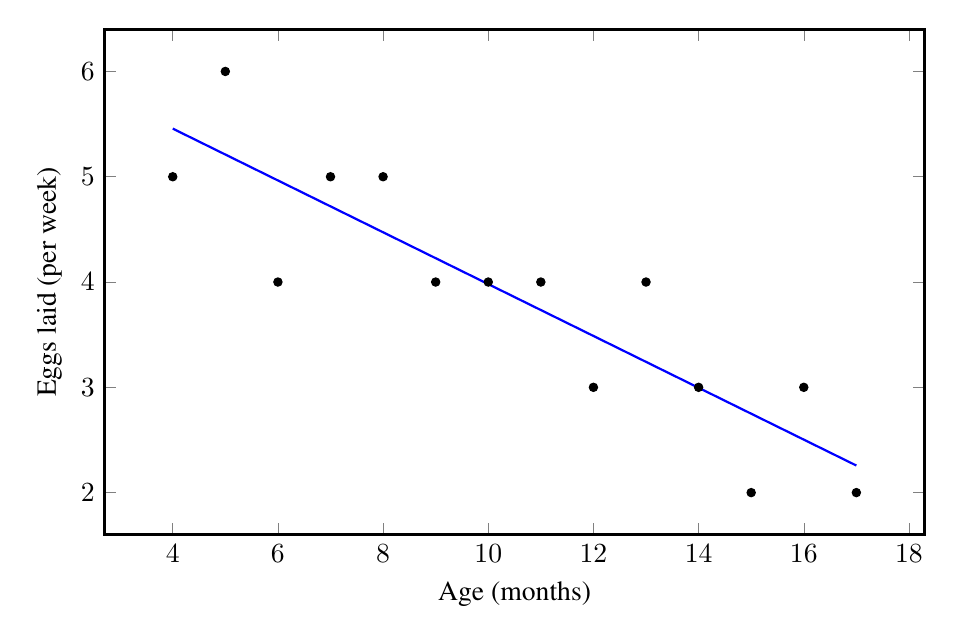
\begin{tikzpicture}
\tikzset{%%
  every mark/.append style={scale=1.0},%%
  scale=1.0%%
}
\pgfplotsset{%%
  every axis/.append style={font=\normalsize}%%
}
%%
\begin{axis}[%%
  axis line style=very thick,%%
  dotStyle/.style={only marks,mark size=1.5,black,mark color=black,mark=*},%%
  enlargelimits=true,%%
  height=8cm,%%
  plotStyle/.style={%%
    domain=4:17,%%
    mark=none,%%
    smooth,%%
    thick%%
  },%%
  width=12cm,%%
  xlabel={\normalsize Age~(months)},%%
  ylabel={\normalsize Eggs laid~(per week)}%%
]
%%
%%
\addplot+ [plotStyle]
{-0.246154*x + 6.441758};
%%
\addplot[dotStyle] coordinates {
  (4,5)
  (5,6)
  (6,4)
  (7,5)
  (8,5)
  (9,4)
  (10,4)
  (11,4)
  (12,3)
  (13,4)
  (14,3)
  (15,2)
  (16,3)
  (17,2)
};
\end{axis}
\end{tikzpicture}

\end{document}
